%! Author = chaorn
%! Date = 07.01.23

Log4Shell besitzt ein Bug Branding (siehe Abbildung 1).
Die in dieser Sektion ausgeführten Unterpunkte beschäftigen sich mit dem Ausnutzen des Zero-Day, der Mitigation und mit den Patches, die im Zusammenhang mit der Schwachstelle angeboten und ausgeführt wurden.
\begin{figure}[!htb]\label{fig:log4shell-logo}
    \begin{center}
        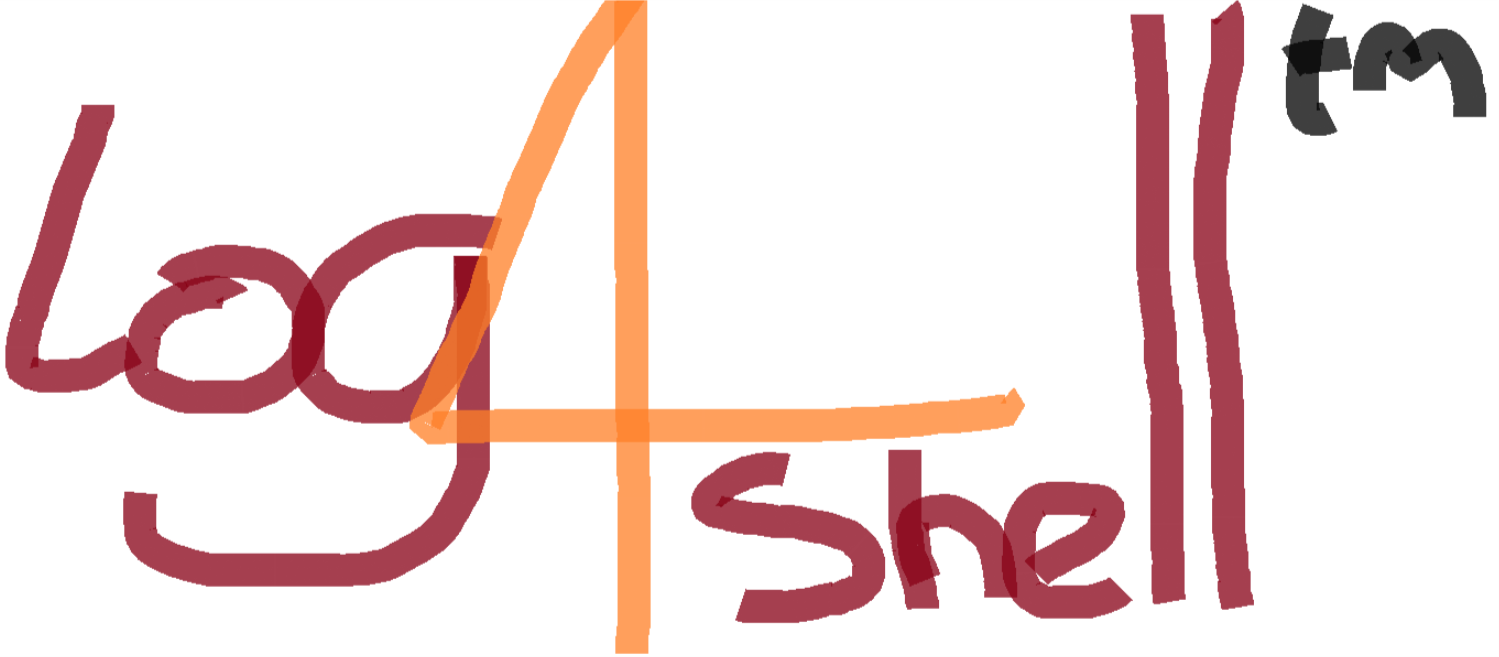
\includegraphics[width=0.3\textwidth]{images/log4shell-logo}
    \end{center}
    \caption{Log4Shell Logo}
\end{figure}

